\section{تغییر مشخصات پانچ ها}

نرم افزار برش پانچ به گونه ای نوشته شده است که تقریبا در تمامی موارد پانچ ستونها را بدرستی تشخیص داده و نسبت آنها را محاسبه میکند. با این حال برای اینکه کاربر بتواند کنترل بیشتری روی 
پارامترهای مختلف محاسبه پانچ داشته باشد، ارتفاع فنداسیون، مقاومت بتن فنداسیون، ابعاد ستونها و موقعیت ستونها در نرم افزار قابل ویرایش هستند.
با تغییر هر یک از پارامترها پانچ تمامی ستونها مجددا محاسبه میشود. ممکن است ستونی که به صورت کنار شناخته شده است با افزایش ضخامت فنداسیون به صورت گوشه شناخته شود و در نتیجه 
نسبت تنش پانچ آن افزایش یابد!

\subsection{تغییر مشخصات فنداسیون}
ضخامت، کاور و مقاومت بتن فنداسیون را میتوان در نرم افزار تغییر داد. برای این کار کافیست که در محیط سه بعدی نرم افزار روی فنداسیون کلیک کنید. با این کار در جدول سمت چپ با نام
\lr{Combo View}
مشخصات فنداسیون به نمایش در می آید (شکل 
\ref{fig:comboview}
). اگر مشخصات قابل رویت نیست به بخش سوالات متداول مراجعه کنید. 
% \ref{faq:dataview}

\begin{figure}[H]
    \centering
    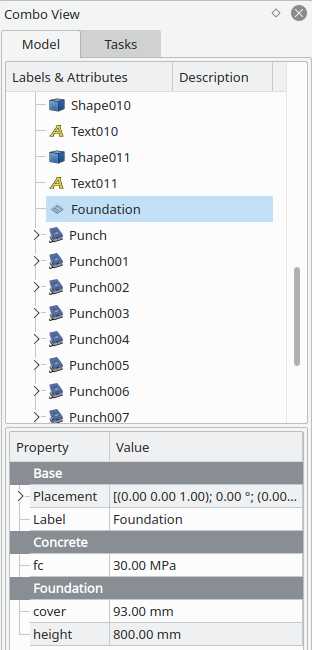
\includegraphics{figures/comboview}
    \caption{تغییر مشخصات فنداسیون}
    \label{fig:comboview}
\end{figure}

\subsection{تغییر مشخصات ستونها}
ابعاد و موقعیت ستونها را میتوان تغییر داد. برای این کار در محیط سه بعدی نرم افزار روی هر کدام از ستونها که قصد تغییر مشخصات آنرا دارید کلیک کنید.
با این کار در جدول سمت چپ مشخصات ستون ظاهر میشود که میتوان ابعاد ستون،
$b_x, b_y$
و موقعیت ستون، 
\lr{Location}
را تغییر داد. برای تغییر ابعاد ستون کافیست که عدد مورد نظر خود را برای ابعاد ستون وارد کنید.
برای تغییر موقعیت ستون ابتدا باید پارامتر 
\lr{user modified}
را از حالت 
\lr{false}
به 
\lr{true}
تغییر دهید و سپس موقعیت جدید ستون را با پارامتر
\lr{Location}
تغییر دهید. دقت کنید که فقط میتوان از پانچ وسط به کنار و گوشه 
و از پانچ کنار به گوشه تغییر موقعیت داد. چون باید صفحات مناسب پانچ برای تشخیص وجود داشته باشد.
یعنی نرم افزار با تغییر موقعیت ستون، یک یا دو صفحه پانچ را حذف میکند، ولی نمیتوان صفحه ای که وجود ندارد را به آن اضافه نمود!

\begin{itemize}
    \item نکته: بجای اینکه ویرایش را جدول کنار نرم افزار انجام دهید میتوانید با دابل کلیک روی اسم هر کدام از پانچ ها در قسمت بالایی جدول
    \lr{Combo View}
    این کار را انجام دهید. پس از دابل کلیک روی نام پانچ مورد نظر، یک پنجره مطابق شکل
    \ref{fig:columnedit}
    باز میشود که میتوانید موقعیت و ابعاد ستون را در آن تغییر دهید. در این پنجره نیز برای تغییر موقعیت ستون تیک مورد نظر را بزنید.
\end{itemize}

\begin{figure}[H]
    \centering
    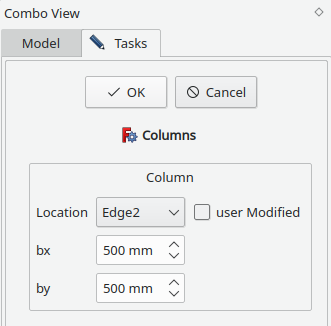
\includegraphics{figures/columnedit}
    \caption{پنجره تغییر مشخصات ستون}
    \label{fig:columnedit}
\end{figure}
